\subsection{Usar el complemento georreferenciador}

El complemento georreferenciador permite generar archivos de referenciación (world files) para rásters. Para ello
se seleccionan puntos en el ráster y se añaden sus coordenadas y el complemento procesa los parámetros del archivo 
de referenciación. Cuantas más coordenadas se proporcionen mejor será el resultado.

Como ejemplo generaremos un archivo de referenciación para una hoja topográfica de Dakota del Sur 
desde SDGS. Más tarde se puede visualizar junto con los datos de la localización  
spearfish60 de GRASS. Puede descargar la hoja topográfica aquí: \\
\url{http://grass.osgeo.org/sampledata/spearfish\_toposheet.tar.gz}

Como primer paso descargamos el archivo y los descomprimimos.

\begin{verbatim}
wget http://grass.osgeo.org/sampledata/spearfish_toposheet.tar.gz
tar xvzf spearfish_toposheet.tar.gz
cd spearfish_toposheet
\end{verbatim}

El siguiente paso es iniciar QGIS, cargar el complemento georreferenciador y seleccionar el archivo spearfish\_topo24.tif.

\begin{figure}[ht]
\begin{center}
  \caption{Seleccionar una imagen a georreferenciar}\label{fig:select_image}\smallskip
  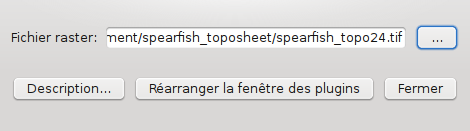
\includegraphics[clip=true,width=0.7\textwidth]{select_image}
\end{center}
\end{figure}

Ahora pulse el botón \textsl{Ajustar ventanas de complementos} para abrir la imagen 
en el georreferenciador y ajustarla en su escritorio con la vista del mapa de referencia en QGIS.

\begin{figure}[ht]
\begin{center}
  \caption{Ajustar la ventana del complemento con la vista del mapa de QGIS}\label{fig:georeferencer}\smallskip
  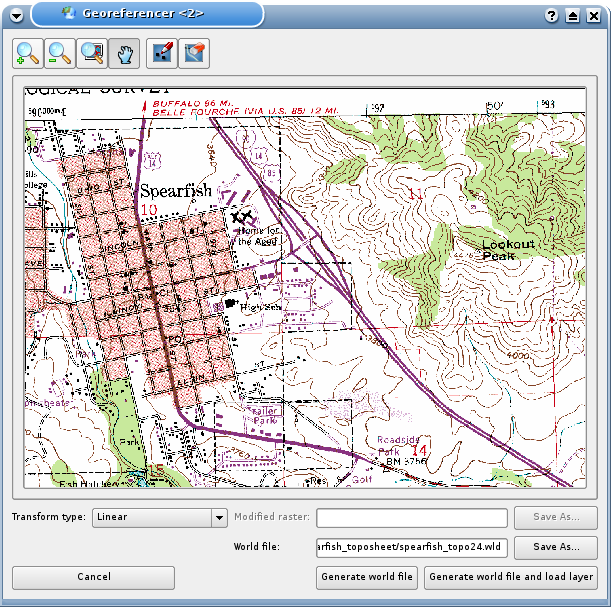
\includegraphics[clip=true,width=\textwidth]{georeferencer}
\end{center}
\end{figure}

Con el botón \textsl{Añadir punto} puede comenzar a añadir puntos en la
imagen ráster e introducir sus coordenadas y el complemento procesará los 
parámetros del archivo de referenciación (vea la Figura \ref{fig:choose_points}). Cuantas más 
coordenadas proporcione mejor será el resultado. Hay dos opciones para el procedimiento:

\begin{enumerate}
\item Pulse en un punto del mapa ráster e introduzca las coordenadas X e Y manualmente.
\item Pulse en un punto en el mapa ráster y seleccione el botón
\textsl{de la vista del mapa} para añadir las coordenadas X e Y con la ayuda de un mapa georreferenciado ya cargado en QGIS.
\end{enumerate}

\begin{figure}[ht]
\begin{center}
  \caption{Añadir puntos a la imagen ráster}\label{fig:choose_points}\smallskip
  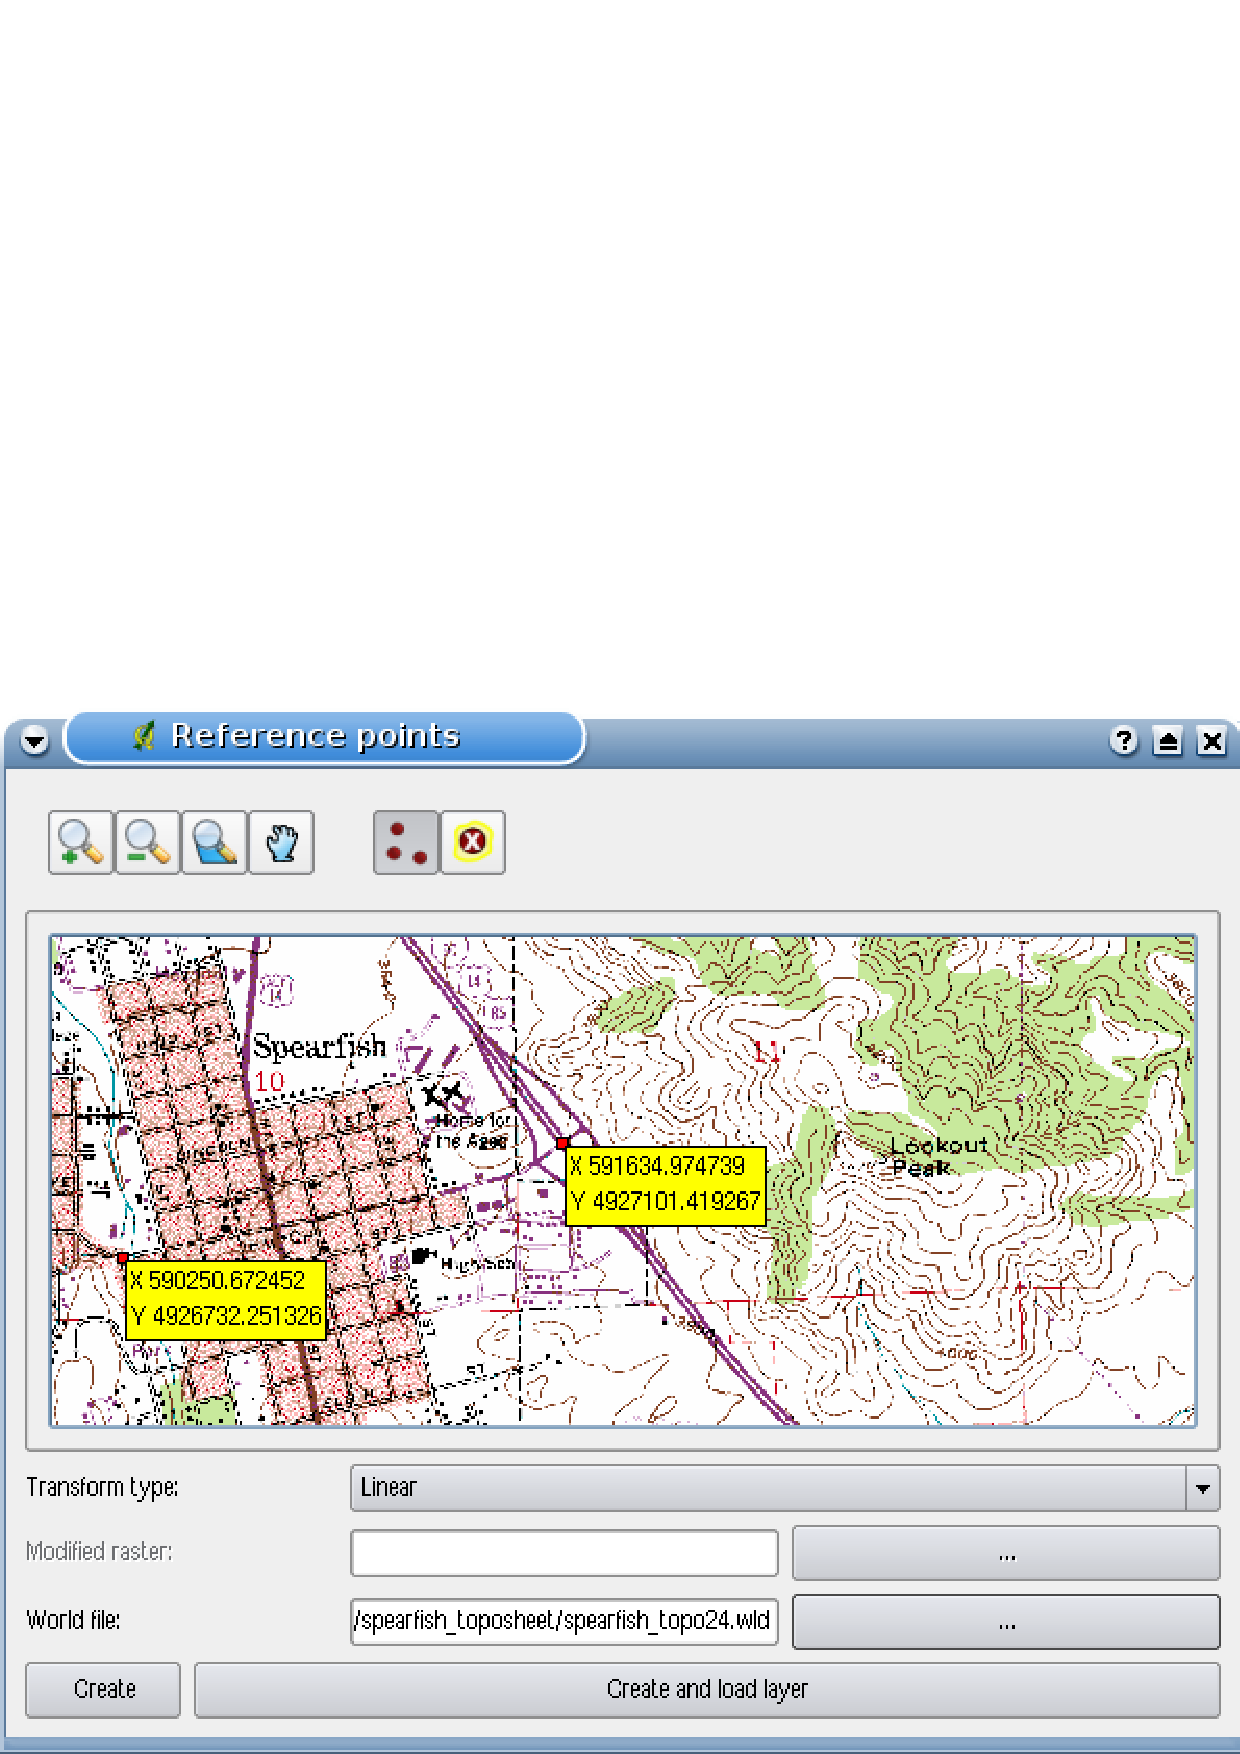
\includegraphics[clip=true,width=0.8\textwidth]{choose_points}
\end{center}
\end{figure}

Para este ejemplo usamos la segunda opción e introducimos las coordenadas de los
puntos seleccionados con la ayuda del mapa \textsl{roads} proporcionado con la 
localización \textsl{spearfish60} de: \\
\url{http://grass.osgeo.org/sampledata/spearfish\_grass60data-0.3.tar.gz}

Si no sabe como integrar la localización spearfish60 con el complemento de GRASS, se da información el la Sección \ref{sec:grass}. 

Como puede ver en la Figura \ref{fig:choose_points}, el georreferenciador proporciona botones 
para hacer zum, panorámica, añadir y borrar puntos en la imagen.

Después de añadir suficientes puntos a la imagen necesita seleccionar el tipo de transformación 
para el proceso de georreferenciación y guardar el archivo de referenciación resultante junto con el 
Tiff. En nuestro ejemplo elegimos transformación lineal, aunque una transformación Helmert también podría valer.

\begin{Tip}\caption{\textsc{Seleccionar el tipo de transformación}}
\qgistip{La transformación lineal (afín) es una transformación de primer orden y se usa para el escalado, 
translación y rotación de imágenes geométricamente correctas. Con la transformación Helmert 
simplemente se añade información de coordenadas a la imagen como geocódigo. Si su imagen está retorcida 
necesitará usar software que proporcione transformaciones polinomiales de segundo y tercer orden, por ejemplo GRASS GIS.
}
\end{Tip} 

Los puntos que añadimos al mapa se guardarán en un archivo \textsl{spearfish\_topo24.tif.points} 
junto con la imagen ráster. Esto nos permite volver a abrir el complemento de georreferenciación y añadir 
puntos nuevos o borrar existentes para optimizar el resultado. El archivo \textsl{spearfish\_topo24.tif.points} de este ejemplo muestra los puntos:

\begin{verbatim}
mapX    		mapY    		pixelX  pixelY
591630.196867999969982  4927104.309682800434530 591647  4.9271e+06
608453.589164100005291  4924878.995150799863040 608458  4.92487e+06
602554.903929700027220  4915579.220743400044739 602549  4.91556e+06
591511.138448899961077  4915952.302661700174212 591563  4.91593e+06
602649.526155399973504  4919088.353569299913943 602618  4.91907e+06
\end{verbatim} 

Hemos usado 5 puntos para georreferenciar la imagen ráster. Para conseguir resultados correctos 
es importante separar los puntos de forma regular por la imagen. Finalmente comprobamos el resultado 
y cargamos el nuevo mapa georreferenciado \textsl{spearfish\_topo24.tif} y lo superponemos con el mapa 
 \textsl{roads} de la localización spearfish60.

\begin{figure}[ht]
\begin{center}
  \caption{Mapa georreferenciado con carreteras superpuestas de la localización spearfish60}\label{fig:result_map}\smallskip
  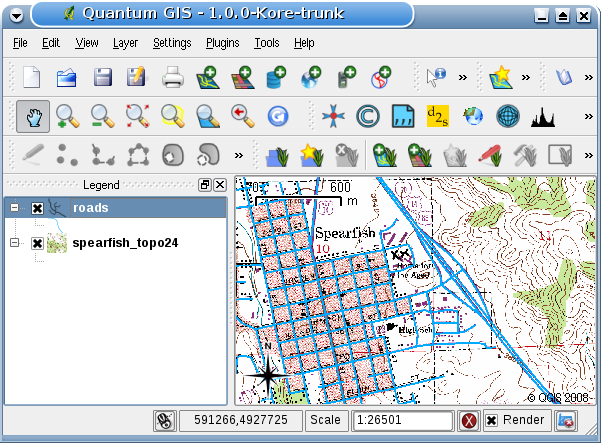
\includegraphics[clip=true,width=0.8\textwidth]{result_map}
\end{center}
\end{figure}







